\documentclass{article}
\usepackage{fullpage,abstract,hyperref,graphicx,caption}
\usepackage{amsmath,amsfonts,amssymb,amsthm,program,float,multirow}

\makeatletter

\newfloat{algorithm}{thp}{lop}
\floatname{algorithm}{Algorithm}

\title{\vspace{-60pt}CS 6491 - Project 3 - 3D Sculpting}

\author{
\begin{tabular}{rr}
&\multirow{3}{*}{\includegraphics[scale=0.4]{chris.jpg}}\\
Christopher Martin\\
\texttt{chris.martin@gatech.edu}&
\end{tabular}
\begin{tabular}{ll}
\multirow{3}{*}{\includegraphics[scale=0.4]{sabri.jpg}}\\&
Sabri Gokmen\\&\texttt{sabrigokmen@gatech.edu}\end{tabular}
~\\~\\~\\}

\newcommand\screenshot[1]{\includegraphics[scale=0.22]{#1}}
\newcommand{\argmin}{\operatornamewithlimits{argmin}}
\newcommand{\argmax}{\operatornamewithlimits{argmax}}
\def\p{\hspace{0pt}}

\begin{document}

\makeatletter
\twocolumn[
\begin{@twocolumnfalse}
\maketitle

\begin{abstract}

We built a virtual environment using a first-person shooter
mechanic which allows a user to sculpt a static three-dimensional
shape by adding and removing spheres.
A triangle mesh is constructed around the spheres to
create the appearance of a solid object.

~\\
\end{abstract}
\end{@twocolumnfalse}
]
\makeatother

\section{Model}

The underlying data structure being manipulated by the user's
actions is simply a set of points, where a point is a tuple of
three floating point numbers denoting the position of a ball
in the model space.
Once placed, each ball's position is fixed.
Balls may be added or removed, but they do not move.
Figure \ref{fig:balls} shows a sample ball arrangement.

\begin{figure}[h!]
\centering
\screenshot{balls}
\caption{The debugging view of the application,
toggled by pressing the \texttt{B} key, shows the
positions of the balls in the model.
In this example, we have started with a pregenerated
``wall'' shape and performed some addition and removal
upon it.}
\label{fig:balls}
\end{figure}

\texttt{W}, \texttt{A}, \texttt{S}, and \texttt{D} keys
move the camera within the model space, and mouse
movement adjusts the camera's orientation.

\section{Spraying}

While the primary mouse button is depressed, balls
are added to the model as if they were produced from
a spray gun pointed directly forward at the center
of the screen.
To determine the trajectory of each ball, we start
with the camera target, and then apply two rotations
as illustrated by Figure \ref{fig:cone}.

\paragraph{Rotation 1}
The point is rotated around an arbitrary line
that passes through the camera point and is
orthogonal to the camera's line of sight.
The angle of rotation is selected randomly on
the range $[0,s]$ where $s$ is the maximum spread.
This spreading parameter can be adjusted at runtime
using the mouse scroll wheel.

\paragraph{Rotation 2}
The point is then rotated around the camera's
line of sight.
This rotation angle is selected uniformly at random
over $[0, 2\pi]$.\\

\begin{figure}[h!]
\centering
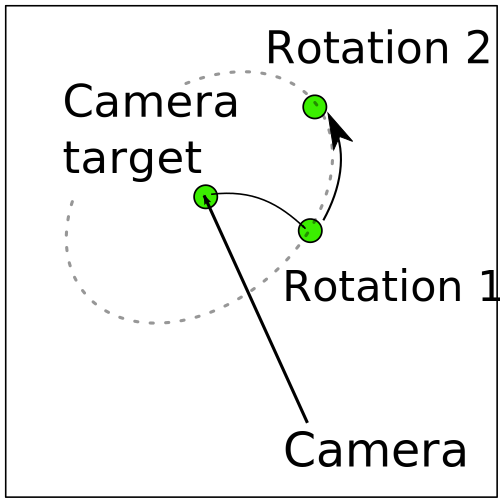
\includegraphics[scale=0.3]{cone}
\caption{Diagram of the strategy for selecting
the direction of a sprayed ball.}
\label{fig:cone}
\end{figure}

Once this point is selected, we now have a ray along
which we can simulate the ball's travel.
We find the closest ball with which the ray collides,
and position a new ball snugly in a corner where it
is in contact with the collided ball and two others.

When an alternate mouse button is pressed, we perform
the same ray selection process, and then remove the
first ball with which the ray collides.

\section{Mesh}

A daemon thread continually generates new triangle
meshes as the ball configuration changes.

\begin{figure}[h!]
\centering
\screenshot{mesh}
\caption{The triangle mesh resulting from the ball
configuration of Figure \ref{fig:balls}.}
\label{fig:mesh}
\end{figure}

For mesh generation, we consider each ball to be
a point located at its center, and then simulate
rolling a testing sphere (having three times the radius
of the balls in the model) around the points,
adding a triangle surface whenever the sphere
comes into contact with three points.

The process begins with the vertex having the
topmost position on the Z axis. The testing sphere is
then iteratively rotated around that point in a downward
spiral until it collides with another point.
The two points and the position of the testing sphere
are added to a worklist of edges that yet need to be
explored.
Then we repeat until the worklist is empty:
\begin{itemize}
\item Pop an edge $(a,b)$ from the worklist.
\item Rotate the testing sphere around the edge until
      it collides with vertex $c$.
\item Add triangle $(a,b,c)$ to the mesh.
\item Add each edge $(a,c)$ and $(c,b)$ to the worklist
      if it does not already belong to another triangle.
\end{itemize}

To capture multiple disconnected components, we
re-run this algorithm until all vertices have
been visited.

\end{document}

